\documentclass[11pt]{article}
\usepackage[a4paper,margin=1in]{geometry}
\usepackage{booktabs}
\usepackage{array}
\usepackage{enumitem}
\usepackage{tikz}
\usetikzlibrary{positioning}
\usepackage{pgfplots}
\pgfplotsset{compat=1.18}
\usepackage{hyperref}
\hypersetup{colorlinks=true,linkcolor=black,urlcolor=blue}

\title{\textbf{Competition Report}\\
Chest X-ray Classification}
\author{Ersa}
\date{}

\begin{document}
\maketitle

\section*{1. Overview}
This project targets 5-class chest X-ray classification using a dense-only neural network design. The final model uses a patch-based representation of the image and mixes information across patches and channels through MLP-style blocks. The main objective was to improve macro F1-score while keeping the training and inference process reliable.

\section*{2. Final Model Idea}
The final architecture follows this flow:
\begin{itemize}[leftmargin=1.2em]
\item Convert input image to grayscale and normalize.
\item Resize to a fixed working size and split into non-overlapping patches.
\item Apply a shared dense projection to each patch.
\item Add learnable positional embeddings so the model keeps spatial context. 
\item Use token-mixing and channel-mixing MLP blocks with skip connections. I got this idea of skipping connections and channel-mixing from this \href{https://github.com/jeonsworld/MLP-Mixer-Pytorch/blob/main/README.md}{Github repo}.
\item Aggregate features with global pooling and predict with a final softmax layer. silhouette within the chest.
\end{itemize}

This design was chosen to capture both local texture and global chest structure without convolution. Since I was considering the problem in a medical context, the changes needed to be visible to the naked eye and primarily involve global features. For example, large-scale changes such as consolidation or an enlarged cardiac 

\section*{3. Training Strategy and Improvements}
Key ideas that improved the score:
\begin{itemize}[leftmargin=1.2em]
\item \textbf{Multi-network in parallel:} I tried this strategy, but it did not lead to a significant improvement in the F1 score; therefore, I decided to omit the use of multiple layers. To be more accurate, I focused on downsampling within each network (each branch of Multi-network in parallel) so that each network would see a more diverse subset of the samples. In this setup, each parallel network was designed to have the same number of samples for each class. In theory, this approach should have worked well; however, it did not produce the expected results. This may be due either to an incorrect implementation on my part or to limitations inherent to the idea itself. I tested this approach at the end of the competition (last day) using a simple r network for each branch and added additional dropout and regularization to mitigate overfitting, but the performance still did not improve.
\item \textbf{Class-aware training:} Class-balanced sampling and class weighting were used to reduce collapse on minority classes.\\ My approach started by increasing the frequency of class~5 samples within each batch, effectively enforcing aggressive class balancing so that all classes were equally represented during training. In theory, this should have helped the network pay more attention to the rare class; however, in practice, performance plateaued and could not be improved further. This led to a clear trade-off between \emph{“pay attention to the rare class”} (via class weighting and oversampling) and \emph{“do not memorize it”} (via regularization and dropout). As shown in the Results section, the model performs reasonably well on the training set—though it clearly overfits on class~5—but generalizes poorly to the validation set. Specifically, the F1 score for class~5 drops from 0.3849 during training to 0.1548 on validation, which is significantly worse compared to other classes and indicates strong overfitting. Increasing the dropout rate helped reduce memorization of class~5, but at the cost of degrading performance across the other classes, leading to an overall loss in accuracy. This trade-off dominated the model development process, and approximately 90\% of the total effort was spent attempting to balance these competing effects.\\
I believe this stage became the main bottleneck of the model. It is likely that the winner of the competition relied on a more effective strategy at this step.\\

\textbf{More technical view of my final setting:}
\begin{itemize}[leftmargin=1.2em]
\item I used \texttt{BALANCE\_TEMPERATURE = 0.6} in the balanced data pipeline. The sampling probability per class is proportional to
\[
P(c)\propto n_c^{\,T}, \quad T=0.6
\]
where \(n_c\) is the number of samples in class \(c\).  
Interpretation: \(T=1\) keeps the original class distribution, \(T=0\) makes all classes equally likely, and \(0<T<1\) is a partial-balance regime.  
So \(T=0.6\) was my compromise between full balancing and the original data distribution.
\item I also used \texttt{CLASS\_WEIGHT\_MAP = \{0:1.0, 1:1.1, 2:1.0, 3:1.05, 4:1.7\}}.  
Apparently this modifies the loss, as
\[
\mathcal{L}=\frac{1}{N}\sum_{i=1}^{N} w_{y_i}\,\mathrm{CE}(y_i,\hat{y}_i),
\]
so errors on class~5 (\(w=1.7\)) contribute much more than errors on majority classes. If I explain this using what we learned in NN class last semester, the way I interpret it is that class weighting effectively changes the gradient landscape: it creates “steeper slopes” toward learning the higher-weight classes. But if the weight is too large, like the large cross-entropy weight I used for class 5, it can also push the model to overfit that class.

\item In practice, these two mechanisms worked together: sampling made minority examples appear more often, and class weights amplified their gradient signal. This improved minority sensitivity, but if pushed too hard, it also increased overfitting risk on class~5.
\end{itemize}

\item \textbf{F1-driven monitoring:} Custom callbacks were used to report per-class F1 scores for both the training and validation sets, which made weak classes visible early in the training process. This allowed me to monitor overfitting per-class and directly compare each class’s training F1 with its corresponding validation F1.

\item \textbf{Mild augmentation:} Horizontal flipping and small rotations were used as data augmentation techniques to improve robustness without excessively distorting medically meaningful patterns. While the precise impact of these augmentations is not entirely clear to me, results showed that horizontal flipping in particular was beneficial, which is reasonable given the left–right symmetry commonly present in X-ray images.

\item \textbf{Stable optimization:} AdamW with LR scheduling and early stopping helped keep training stable.  
I used \texttt{ReduceLROnPlateau} with factor \(0.5\), patience \(=5\), and \(\texttt{min\_lr}=10^{-6}\), monitored on validation macro-F1.  
When validation F1 stopped improving for several epochs, the learning rate was reduced by half:
\[
\eta \leftarrow 0.5\,\eta .
\]
This was useful for two reasons: first, the model could learn quickly in early epochs with a larger step size; second, once it reached a plateau, smaller steps helped avoid oscillation and improved convergence along the smaller eigenvalues . This is similar to the lab we saw in NN class, where a large learning rate causes the optimization to fluctuate perpendicular to the dominant gradient contour lines.   
Without this scheduler, I repeatedly observed unstable late-epoch behavior, especially under imbalance-aware training. I realized the learning rate scheduler matters when the problem becomes complicated, like deep learning networks.
\end{itemize}

\section*{4. Results}
\subsection*{4.1 Per-Class F1 (Current Run)}
\begin{center}
\begin{tabular}{lcc}
\toprule
\textbf{Class} & \textbf{Train F1} & \textbf{Validation F1} \\
\midrule
Class 1 & 0.4462 & 0.4330 \\
Class 2 & 0.3962 & 0.3070 \\
Class 3 & 0.5044 & 0.3968 \\
Class 4 & 0.4508 & 0.3159 \\
Class 5 & 0.3849 & 0.1548 \\
\midrule
\textbf{Macro F1} & \textbf{0.4365} & \textbf{0.3215} \\
\bottomrule
\end{tabular}
\end{center}

\subsection*{4.2 Final Test Metric}
\begin{itemize}[leftmargin=1.2em]
\item Test macro F1-score:  \textbf{0.3449}
\item Competition F1-score: \textbf{0.327}
\end{itemize}

\subsection*{4.3 F1 Visualization}
\begin{center}
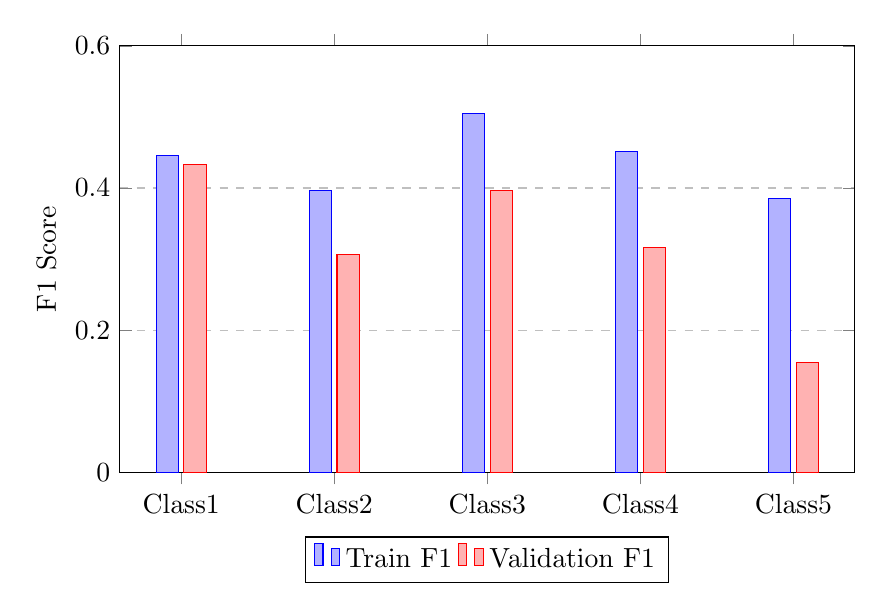
\begin{tikzpicture}
\begin{axis}[
    ybar,
    bar width=8pt,
    width=0.9\textwidth,
    height=7cm,
    ymin=0, ymax=0.6,
    ylabel={F1 Score},
    symbolic x coords={Class1,Class2,Class3,Class4,Class5},
    xtick=data,
    legend style={at={(0.5,-0.15)},anchor=north,legend columns=2},
    ymajorgrids=true,
    grid style=dashed,
]
\addplot coordinates {(Class1,0.4462) (Class2,0.3962) (Class3,0.5044) (Class4,0.4508) (Class5,0.3849)};
\addplot coordinates {(Class1,0.4330) (Class2,0.3070) (Class3,0.3968) (Class4,0.3159) (Class5,0.1548)};
\legend{Train F1, Validation F1}
\end{axis}
\end{tikzpicture}
\end{center}

\section*{5. Architecture Diagram (High Level)}
\begin{center}
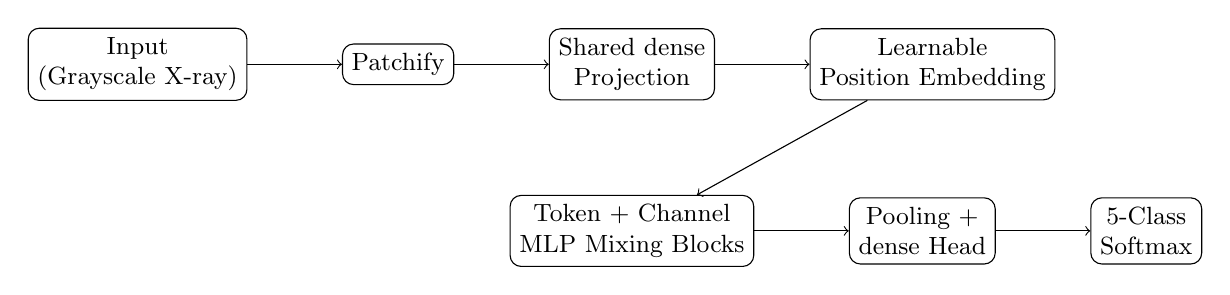
\begin{tikzpicture}[node distance=1.2cm, every node/.style={font=\small}]
\node[draw, rounded corners, align=center] (in) {Input\\(Grayscale X-ray)};
\node[draw, rounded corners, align=center, right=of in] (patch) {Patchify};
\node[draw, rounded corners, align=center, right=of patch] (proj) {Shared dense\\Projection};
\node[draw, rounded corners, align=center, right=of proj] (pos) {Learnable\\Position Embedding};
\node[draw, rounded corners, align=center, below=of proj] (mix) {Token + Channel\\MLP Mixing Blocks};
\node[draw, rounded corners, align=center, right=of mix] (head) {Pooling +\\dense Head};
\node[draw, rounded corners, align=center, right=of head] (out) {5-Class\\Softmax};

\draw[->] (in) -- (patch);
\draw[->] (patch) -- (proj);
\draw[->] (proj) -- (pos);
\draw[->] (pos) -- (mix);
\draw[->] (mix) -- (head);
\draw[->] (head) -- (out);
\end{tikzpicture}
\end{center}
In the final implementation, I used the following components and each one had a specific role:
\begin{itemize}[leftmargin=1.2em]
\item \textbf{Resize to \(120\times120\)} --- {Why:} reduce memory/computation while keeping global chest anatomy visible.
\item \textbf{\(8\times8\) non-overlapping patches (\(225\) tokens)} --- {Why:} convert the image into local regions so dense layers can learn local-to-global patterns.
\item \textbf{Shared dense projection to 128 dims} --- {Why:} learn a compact feature representation per patch with shared parameters.
\item \textbf{Learnable positional embedding} --- {Why:} preserve location context (upper/lower lung, heart region, diaphragm area). I had this idea but I could not implement it, so I relied on AI. However, I did not fully understand the resulting approach, and I was unable to properly validate the code by AI. 
\item \textbf{3 mixer blocks} --- {Why:} enough depth for feature interaction without making optimization unstable.
\item \textbf{Token-mixing MLP (64 hidden)} --- {Why:} exchange information across patches (global structure reasoning).
\item \textbf{Channel-mixing MLP (256 hidden)} --- {Why:} enrich feature transformation within each patch token.
\item \textbf{Dense-style skip connectivity (concat + projection)} --- {Why:} improve gradient flow, reuse earlier features, and stabilize training.
\item \textbf{Global average pooling} --- {Why:} summarize token-level information into one image-level descriptor. I just love average and max pooling. 
\item \textbf{Dense(256) + Dropout + Softmax(5)} --- {Why:} final nonlinear decision layer, regularization, and class probability output.
\end{itemize}

\section*{6. Discussion}
The best gains came from combining three elements: (1) patch-based dense modeling with positional information, (2) class-aware training for imbalance, and (3) per-class F1 monitoring for targeted iteration. This workflow improved macro F1 and made failure modes clearer, especially for hard minority cases. 

\section*{7. Conclusion}
The final system achieved competitive macro F1 with a compact and interpretable dense-only design. Future gains are likely from better minority-class generalization and calibration.

\section*{8. Fun Note}
One funny point about my nickname \textbf{Ersa}: Named by Twitter Contest. :) \\In 2019, the Carnegie Institution for Science ran a Twitter naming contest for five newly discovered moons of Jupiter. Specifically a school in Canada, suggested Ersa, which was approved by the International Astronomical Union.\\




\end{document}
